\documentclass[a4paper,11pt,twocolumn]{article}

\usepackage{icphs2023}
\usepackage{metalogo} % Only needed for the XeLaTeX logo
\usepackage{epstopdf}
\usepackage{tipa} %
\newcommand{\ipa}{\textipa}
\usepackage{amsmath}% http://ctan.org/pkg/amsmath
\newcommand{\argmax}{\mathop{\rm arg~max}\limits}
\newcommand{\argmin}{\mathop{\rm arg~min}\limits}
\usepackage{svg}

\hyphenpenalty=10000 % no hyphenation
% https://docs.google.com/document/d/1df4t0mZm1gUytgQOYaZNg6-mcneA4knqTvUPMIhoMMc/edit?usp=sharing
% https://docs.google.com/document/d/1VywiSaEORlVrRDb7nxGQx2D0pu6huftZrEiVQKmCGWY/edit?usp=sharing

\title{The role of allophones in phoneme perception models: Do devoiced vowels trigger vowel epenthesis?}
% \name{
\author{
    Takeshi Kishiyama$^1$,
    Chuyu Huang$^2$,
    Kei Furukawa$^3$,
    Yuki Hirose$^1$}
% \address{
\organization{
  $^1$Graduate School of Arts and Sciences, The University of Tokyo, Japan\\
  $^2$Faculty of Foreign Studies, Nagoya Gakuin University, Japan\\
  $^3$Nara Institute of Science and Technology, Japan}
\email{
    kishiyama.t@gmail.com,
    huang@ngu.ac.jp,
    furukawa.kei.fi4@is.naist.jp,
    hirose@boz.c.u-tokyo.ac.jp
    }
\begin{document}

\maketitle

\begin{abstract}
This study investigated how phoneme perception models should incorporate allophones, leveraging dialectical differences among Japanese. It has been reported that listeners of a language that disallows consonant clusters insert epenthetic vowels, or illusory vowels, to repair illegal consonant clusters, thus, for example, perceiving VCCV as VCVCV. In addition to the roles of phonotactic constraints and acoustic cues, recent studies have indicated that allophones, such as devoiced vowels in the Tokyo dialect, also facilitate perceptual epenthesis. We compared the discrimination accuracies of VCCV and VCVCV perception of Tokyo-dialect speakers to those of Kansai-dialect speakers, who are reported to devoice vowels less frequently. Both Tokyo and Kansai speakers perceived illusory vowels to the same degree, indicating that illusory vowels were perceived even by speakers without devoicing. Furthermore, the results suggest that discriminative models other than probabilistic models assuming an auditory realization distribution can be psychologically valid.
\end{abstract}

\keywords{speech perception, phonotactics, context effects, perceptual epenthesis, dialect}

\section{Introduction}

When hearing speech sounds that violate the phonotactics of the native language, the listener perceives the phonemes according to the rules. For example, native Japanese speakers perceive [ebzo] as /ebuzo/ according to their phonotactics. The \textit{illusory vowel} is perceptually inserted for stimuli where the vocal fold vibration of the vowel is acoustically absent \cite{dupoux1999epentheticvi, dupoux2011illusory}. Recently, devoicing and allophones have been reported to affect the illusion, and our study reexamined these effects through experiments on dialect speakers and discussed how we should incorporate them into perceptual models.

First, phonotactics provide insights into the vowel illusion \cite{dupoux1999epentheticvi, halle2014special, monahan2009not, mattingley2015influence, guevara2017predicting, guevara2017epenthetic}, as shown in an experiment with native French and Japanese speakers \cite{dupoux1999epentheticvi}. Unlike French, Japanese disallows the consonant cluster /bz/, and the speakers of each language tried to discriminate between [ebuzo] and [ebzo] in the experiment. While French speakers successfully distinguished them, Japanese speakers perceived [ebzo] as /ebuzo/, which decreased their discrimination accuracy.

In addition to the phonotactics, experiments with native speakers of Brazilian Portuguese and Japanese have revealed the influence of acoustic cues on illusory vowels \cite{dupoux2011illusory}. Both languages do not allow /bz/, and the default vowels to be inserted are /i/ and /u/, respectively. The study deleted the vowels between /b/--/z/ in [ebizo] and [ebuzo], leaving the vowels' acoustic cues in /b/. The remained cues affected the subjects of both languages, increasing the insertion rate of the non-default /i/ for Japanese.

Based on these results, previous research has assumed one-step models, where phonotactics and acoustic cues affect the illusion simultaneously. The one-step models can be represented by hidden Markov models (HMMs), which can also represent perceptual assimilation models \cite{best2001discrimination} and models in exemplar theory \cite{lacerda1995perceptual}, having reproduced the illusory vowels \cite{kishiyama2021influence} by calculating Equation 1. The equation calculates two likelihoods: $P(c|c_{t-1})$ represents the likelihood of the phoneme array $c_{t-1}$ to $c$, and $P(S_{\text{new}}|c)$ represents the likelihood of the input speech $S_{\text{new}}$ for a phoneme $c$. Consequently, the phoneme $c$ that maximizes the likelihoods is activated as $\hat{c}$.
% no break
\begin{equation} \label{hmm}
    \hat{c} = \argmax_{c} P(c | c_{t-1})P(S_{\text{new}}|c)
\end{equation}
% no break
Traditionally, the unit assumed as $c$ above was phonemes \cite{wilson2013bayesian}. Recent studies, however, have suggested that allophones should be treated as discrete units in perceptual models.

First, devoiced/deleted vowels in Japanese are reported to increase the perceptual epenthesis \cite{kilpatrick2018japanese}. Tokyo-dialect in Japanese deletes the high vowel /u/ in /esupo/, and it would be [espo] when the vowel follows fricatives or affricates \cite{fujimoto2003devoice_eng, shaw2018lingual}. In other cases, the vowel in /epuso/ becomes devoiced as [ep\textsubring{\textturnm}so]. The study reported that the deletion/devoicing encouraged assimilation and increased the perceptual epenthesis. Furthermore, transition probabilities between allophones are reported to cause vowel illusion \cite{kilpatrick2020japanese}. Japanese [\textctc], a realization of /s/, precedes /i/ but not other vowels. The study investigated whether [\textctc{}] induces the illusion of /i/ more \cite{kilpatrick2020japanese} and found that the /i/ was perceived more frequently after [\textctc] than after [g]. This result suggests that allophones and their transition probabilities affect the vowel illusion.

The question is whether phoneme perception models should consider allophones categorical rather than continuous. Without the assumption of categorical allophones, the one-step models can explain the results above. The difference in the auditory cues within the deleted and devoiced vowels yield different $P(S_{\text{new}}|c)$ in Eq. (1). Furthermore, the stimuli [\textctc] is supposed to have acoustic cues of /i/ \cite{kubozono1999japanese_eng}, which can also change $P(S_{\text{new}}|c)$ in Eq. (1). To explain the results, therefore, the models do not need to have categorical allophones.

What allows multiple interpretations for the experiments is the confounding of the allophones and the acoustic cues, and we leveraged dialectal differences between the Kansai and Tokyo dialects in Japanese \cite{kishiyama2022onestep}. First, in [ep\textsubring{\textturnm}so] and [espo], not only the allophones (devoiced/deleted) but also the preceding speech sounds ([p]/[s]) are different. In addition, in comparisons of [egpo] and [e\textctc{}po], the transition probability from [g] or [\textctc] to the next vowel is confounded with the acoustic cues of [g] or [\textctc]. We can deal with this issue using the Kansai dialect speakers, who tend to devoice/delete vowels less frequently than the Tokyo dialect speakers do \cite{byun2011_eng, byun2012_eng}. According to the assumption that the deletion and devoicing caused the illusion, the Kansai-dialect speakers, who are less exposed to those allophones, should yield few illusions and more accurate responses in discriminative AXB tasks.

\section{Perception experiment}

% FIXME: ナンバリングがなくなっている
\subsection{Materials and methods}

%FIXME: check M and SD
We used an outsourcing service to recruit subjects who were older than 18 years and from Tokyo or the Kansai region, and those who had never lived in other areas since birth had priority in the recruitment process. We had 62 subjects ($M$=40, $SD$=15) while excluding the results of the four subjects whose answers were under 75\% accuracy in the categorization task (\S3).

In the AXB task, the participants were to distinguish between VC$_\text{1}$VC$_\text{2}$V and VC$_\text{1}$C$_\text{2}$V in a list of target stimuli with 32 items based on the combination of the four conditions below. (1) For environments where deletion and devoicing occur, we established four pairs for C$_\text{1}$C$_\text{2}$: s--p, k--t, p--s, and ts--k. (2) We also had stimuli VC$_\text{1}$VC$_\text{2}$V with /u/ between C$_\text{1}$ and C$_\text{2}$ that the participants had to discriminate from VC$_\text{1}$C$_\text{2}$V. (3) We also created two patterns depending on whether a trial's stimulus in the X position was either VC$_\text{1}$VC$_\text{2}$V or VC$_\text{1}$C$_\text{2}$V, which is to be distinguished in the AXB task. (4) We prepared voiced counterparts of C$_\text{1}$ and C$_\text{2}$, such as b--z, where neither deletion nor devoicing occurs. The positions of correct answers were counterbalanced, A or B.

We recorded stimuli from three male speakers and adjusted the loudness to 75 dB. The duration before C$_\text{2}$ was about 50 ms (about 400 ms for the entire three moras) so that the subjects would not perceive a long blank as the "geminate" consonant, a distinctive phoneme \textit{sokuon} in Japanese. We removed the voicing parts of /egudo/ and /ebuzo/ based on formant and power and extended the silent interval. In this case, the cycle of each preceding waveform was duplicated and extended. In contrast, /u/ in /epuso/ was cut so that it would be of the same duration as /epuso/.

After three sets of practice tasks, 32 target and 24 filler items were randomized and presented to the subjects in an experimental environment conducted on web browsers. A "+" was displayed in the center of the screen for 1000 ms before the audio stimuli, and the three audio items were presented at intervals of 200 ms. After the presentation was over, the subject was to respond as quickly as possible. We didn't feed back correct or incorrect to avoid learning during the task, and the program only provided answers in the practice task. When a trial ended, the participants could start the next trial by pressing the space key.

\subsection{Results}

The y-axis in the Figure \ref{fig:axb_results} shows the average discrimination accuracy of VC$_\text{1}$VC$_\text{2}$V and VC$_\text{1}$C$_\text{2}$V in the AXB discrimination task. On the left and right panes, we indicated whether the stimulus was in devoicing environment (e.g., k--t if C$_\text{1}$C$_\text{2}$ was devoicing condition, g--d if not). The x-axis shows the Tokyo--Kansai ratio, the ratio of residential history between Tokyo and the Kansai region. For example, if a subject has lived in Tokyo for 25 years and in Kansai for 15 years, the ratio is $(25-15)/40$, or $0.25$. We showed four items vertically to see tendencies for each item,
\begin{figure}[!ht]
\begin{center}
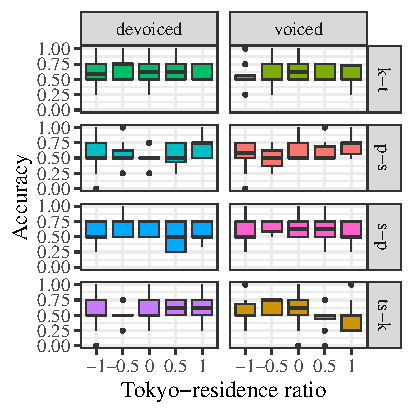
\includegraphics[width=6.5cm]{../results/artifact/results_axb_allophone.pdf}
\caption{A boxplot that shows the relationship between the residential history and perceptual illusion.}\label{fig:axb_results}
\end{center}
\end{figure}

We checked the distribution of the reaction time data and excluded the 0.61\% of data with a reaction time of 10 seconds or longer as outliers. We calculated the mean accuracy, averaging four patterns based on the X in AXB (VC$_\text{1}$VC$_\text{2}$V or VC$_\text{1}$C$_\text{2}$V) and the correct answer position (A or B) and excluding missing values.

% FIXME: add table
We created a Bayesian linear mixed-effects model \cite{lme4, rstanarm, easystats} with the Tokyo--Kansai ratio as the independent variable and the AXB task discrimination accuracy as the dependent variable. Item type and subjects were modeled as random effects. The analysis revealed an overall mean accuracy of 0.59, without consistent effects for environmental. The estimates of dialectal differences were positive (0.019) and not in the direction of decreasing precision.

To evaluate the null hypothesis, we calculated a Bayes factor ($BF$) for the Tokyo--Kansai ratio. The Bayes factor, which is used to compare the models in the framework of Bayesian statistics, was 0.150 and provided substantial evidence for the null hypothesis. In this study, we calculated the $BF$ as $Posterior \text{ }Odds / Prior \text{ }Odds$, where each $Odds$ is calculated as: $P(b\notin[0, \infty] | Data)/P(b\in[0, \infty] | Data)$ and $P(b\notin[0, \infty])/P(b\in[0, \infty])$, respectively. Since $b$, the effect of the Tokyo--Kansai ratio was supposed to be negative, the null region\cite{kruschke2010believe}, considered to have no effect, was set to a positive value [0, $\infty$].

The $BF$ of the Tokyo--Kansai ratio was 0.15, which indicated that the null hypothesis of a positive effect was $1/0.15(=6.67)$ times more plausible than the alternative hypothesis of a negative effect. This result contradicts the interpretation that the allophone increases the rate of illusions and decreases the accuracy.

\subsection{Discussion}

If the allophone creates the illusion of a vowel, the Tokyo dialect speakers with the allophone should have lower accuracy in the discrimination experiment than speakers without devoicing. However, the results of the AXB task showed that the discrimination accuracy of both Kansai and Tokyo dialect speakers, regardless of their language experience, was around 0.59, which is close to a chance level. In addition, the $BF$ suggested that the language experience and devoicing did not affect the rate of illusions in the discrimination task.

Next, the categorization task investigated dialectal differences and acceptability judgments about devoicing in offline processing. We examined whether dialect differences in language experience affect the goodness rating of deletion/devoicing. Note that we performed this categorization task after the online process to avoid any effect on the validation of the online process.

\section{Categorization task}

\subsection{Materials and methods}

The subjects in the perceptual task also participated in this task. All sounds presented in the perceptual task were categorized. There are eight different patterns: four to be devoiced in the Tokyo dialect (esupo, ekuto, epuso, etsuko) and four not to be devoiced (ezubo, egudo, ebuzo, edzugo). Each of them had devoiced version, and the choices were shown in Japanese letters on the screen. Since three speakers recorded 16 patterns, the subjects listened to 48 stimuli.

Subjects listened to the stimuli, selected which of the above eight options shown above was closest to it, and rated its acceptability on a 7-point scale (0--6). In the rating, zero was considered "not appropriate at all," and six was considered "completely appropriate."

\subsection{Results}

% FIXME: make the figure gray-scale
% FIXME: check left/right panes
The x-axis in Figure \ref{fig:cat_results} shows the Tokyo--Kansai ratio, and the y-axis shows the goodness of fit rating. The left and right panes indicate the environment of speech (devoicing or not), and the color difference shows whether the actual stimulus was devoiced or not. The overall ratings were above the mean of 4. The devoiced stimulus was rated higher in the devoiced environment (left pane), while they were rated lower in the no-devoicing environment (right pane). The residential history does not contribute to these differences.
\begin{figure}[!ht]
\begin{center}
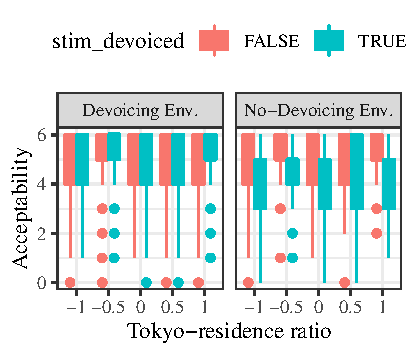
\includegraphics[width=6.5cm]{../results/artifact/results_categorization.pdf}
\caption{A boxplot that shows the relationship between the residential history and the goodness of fit rating.}\label{fig:cat_results}
\end{center}
\end{figure}

To test these points, we created a Bayesian linear mixed-effects model with the goodness of fit rating as the dependent variable. The independent variables were environment (devoicing/no-devoicing), stimulus type (devoiced / not devoiced), the Tokyo--Kansai ratio, and their interactions. Subjects and items were random effects, and we employed a normal distribution ($M=0$, $SD=10$) as a prior distribution for each parameter.

The mean rating was 4.87, indicating that the evaluation was generally natural, given that the rating range was 0--6. The devoicing environment and the devoiced stimulus were $-0.37$ and $-0.79$, respectively. Furthermore, the interaction, i.e., the devoiced stimulus in the devoiced environment, increased the rating by 1.19. The $BF$ for the Tokyo--Kansai ratio was 0.012 when the null region was set to $[-\infty, 0]$, indicating robust evidence of no effect.

\subsection{Discussion}

The results showed that the overall responses were above 4, which means that the quality of the stimuli in this study was not lower than in previous studies \cite{kilpatrick2018japanese}. If the subjects can judge the devoiced speech in the Tokyo dialect offline without epenthesis, the rate of devoiced stimuli in a no-devoicing environment would be less than. The results of the categorization task showed that both Tokyo dialect and Kansai dialect speakers showed that the rating increased when the speech was devoiced in a devoicing environment, while it decreased when the devoiced stimuli were in a no-devoicing environment. However, the effect of the interaction was only about 1, not high enough to cross the threshold between unnatural and natural.

\section{General Discussion}

Previous research proposed that the vowel illusion was caused by devoicing. In addition, probabilistic models included the distribution of auditory realizations. This study proposes a different interpretation based on the results of perceptual experiments and categorization tasks.

First, the results of the discrimination accuracy and categorization tasks in the previous studies were not due to the effect of devoicing but to acoustic differences. Suppose the perceptual epenthesis was due to the devoicing or deletion. In that case, the discrimination accuracy of Tokyo dialect speakers should be lower than that of Kansai dialect speakers who do not devoice or delete the vowels, but there was no such effect. Instead, the Kansai dialect speakers perceived the illusory vowels as the Tokyo dialect speakers do in our study.

Second, regarding how acoustic cues affect speech perception, previous studies \cite{wilson2013bayesian, kishiyama2021influence} have assumed Eq. \ref{hmm} during inference. On the right-hand side, $P(S_{\text{new}}|c)$ is thought to represent the distribution of auditory realizations for phonemes or the perceptual likelihood of $S_{\text{new}}$ given $c$. This formula makes the results consistent with the previous study because $P$( [\textsubring{\textturnm}] | /u/ ) or $P$( [s] | /su/ ) is not zero given that the Kinki dialect speakers hear them since these are in Tokyo-dialect, which are prevalent in Japan. Given Bayes Theorem, the equation can be rewritten as Eq. (\ref{disc}), and it integrates discriminative models.
%
\begin{equation} \label{disc}
    \hat{c} = \argmax_{c} P(c | c_{t-1}) \frac{P(c|S_{\text{new}})}{P(c)}
\end{equation}
%
Thus, it allows us to employ other discriminative models, such as neural networks and multinomial logistic regressions. Since previous studies have already supported the validity of HMMs \cite{kishiyama2021influence}, we will test whether we can incorporate the above discriminative model into HMMs to explain behavioral data.

\bibliographystyle{IEEEtran}

\bibliography{mybib}

\end{document}
